\documentclass{standalone}

\usepackage{graphics}
\usepackage[dvipsnames,svgnames]{xcolor}

\usepackage{tikz,pgf,pgfplots,circuitikz}
\pgfplotsset{compat=1.15}
\usetikzlibrary{intersections,arrows.meta,angles,calc,3d,decorations.pathmorphing}

\usepackage{amssymb,amsfonts,amsthm,mathtools}
\usepackage{physics,braket,bm}

\begin{document}  
  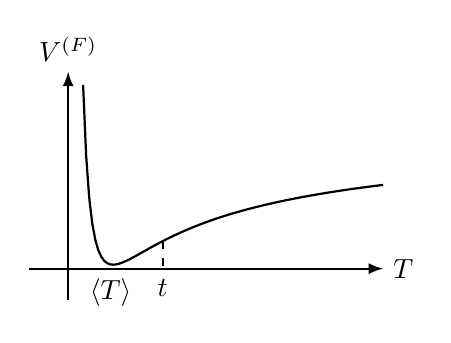
\begin{tikzpicture}[scale=1]
    \draw[-latex,thick](-0.5,0)--(4,0)node[right]{$T$};
    \draw[-latex,thick](0,-0.4)--(0,2.5)node[above]{$V^{(F)}$};
    \draw[thick,samples=100,domain=0.19:4.00]plot(\x,{-ln(5*\x)/(\x)+1/(20*\x)+1.8});    
    \draw (0.51,0)node[below]{$\ev*{T}$};
    \draw[dashed,thick](1.2,0.35)--(1.2,0)node[below]{$t$};
  \end{tikzpicture}
\end{document}
